% Options for packages loaded elsewhere
\PassOptionsToPackage{unicode}{hyperref}
\PassOptionsToPackage{hyphens}{url}
\PassOptionsToPackage{dvipsnames,svgnames,x11names}{xcolor}
%
\documentclass[
  letterpaper,
  DIV=11,
  numbers=noendperiod]{scrreprt}

\usepackage{amsmath,amssymb}
\usepackage{iftex}
\ifPDFTeX
  \usepackage[T1]{fontenc}
  \usepackage[utf8]{inputenc}
  \usepackage{textcomp} % provide euro and other symbols
\else % if luatex or xetex
  \usepackage{unicode-math}
  \defaultfontfeatures{Scale=MatchLowercase}
  \defaultfontfeatures[\rmfamily]{Ligatures=TeX,Scale=1}
\fi
\usepackage{lmodern}
\ifPDFTeX\else  
    % xetex/luatex font selection
\fi
% Use upquote if available, for straight quotes in verbatim environments
\IfFileExists{upquote.sty}{\usepackage{upquote}}{}
\IfFileExists{microtype.sty}{% use microtype if available
  \usepackage[]{microtype}
  \UseMicrotypeSet[protrusion]{basicmath} % disable protrusion for tt fonts
}{}
\makeatletter
\@ifundefined{KOMAClassName}{% if non-KOMA class
  \IfFileExists{parskip.sty}{%
    \usepackage{parskip}
  }{% else
    \setlength{\parindent}{0pt}
    \setlength{\parskip}{6pt plus 2pt minus 1pt}}
}{% if KOMA class
  \KOMAoptions{parskip=half}}
\makeatother
\usepackage{xcolor}
\setlength{\emergencystretch}{3em} % prevent overfull lines
\setcounter{secnumdepth}{5}
% Make \paragraph and \subparagraph free-standing
\makeatletter
\ifx\paragraph\undefined\else
  \let\oldparagraph\paragraph
  \renewcommand{\paragraph}{
    \@ifstar
      \xxxParagraphStar
      \xxxParagraphNoStar
  }
  \newcommand{\xxxParagraphStar}[1]{\oldparagraph*{#1}\mbox{}}
  \newcommand{\xxxParagraphNoStar}[1]{\oldparagraph{#1}\mbox{}}
\fi
\ifx\subparagraph\undefined\else
  \let\oldsubparagraph\subparagraph
  \renewcommand{\subparagraph}{
    \@ifstar
      \xxxSubParagraphStar
      \xxxSubParagraphNoStar
  }
  \newcommand{\xxxSubParagraphStar}[1]{\oldsubparagraph*{#1}\mbox{}}
  \newcommand{\xxxSubParagraphNoStar}[1]{\oldsubparagraph{#1}\mbox{}}
\fi
\makeatother


\providecommand{\tightlist}{%
  \setlength{\itemsep}{0pt}\setlength{\parskip}{0pt}}\usepackage{longtable,booktabs,array}
\usepackage{calc} % for calculating minipage widths
% Correct order of tables after \paragraph or \subparagraph
\usepackage{etoolbox}
\makeatletter
\patchcmd\longtable{\par}{\if@noskipsec\mbox{}\fi\par}{}{}
\makeatother
% Allow footnotes in longtable head/foot
\IfFileExists{footnotehyper.sty}{\usepackage{footnotehyper}}{\usepackage{footnote}}
\makesavenoteenv{longtable}
\usepackage{graphicx}
\makeatletter
\def\maxwidth{\ifdim\Gin@nat@width>\linewidth\linewidth\else\Gin@nat@width\fi}
\def\maxheight{\ifdim\Gin@nat@height>\textheight\textheight\else\Gin@nat@height\fi}
\makeatother
% Scale images if necessary, so that they will not overflow the page
% margins by default, and it is still possible to overwrite the defaults
% using explicit options in \includegraphics[width, height, ...]{}
\setkeys{Gin}{width=\maxwidth,height=\maxheight,keepaspectratio}
% Set default figure placement to htbp
\makeatletter
\def\fps@figure{htbp}
\makeatother
% definitions for citeproc citations
\NewDocumentCommand\citeproctext{}{}
\NewDocumentCommand\citeproc{mm}{%
  \begingroup\def\citeproctext{#2}\cite{#1}\endgroup}
\makeatletter
 % allow citations to break across lines
 \let\@cite@ofmt\@firstofone
 % avoid brackets around text for \cite:
 \def\@biblabel#1{}
 \def\@cite#1#2{{#1\if@tempswa , #2\fi}}
\makeatother
\newlength{\cslhangindent}
\setlength{\cslhangindent}{1.5em}
\newlength{\csllabelwidth}
\setlength{\csllabelwidth}{3em}
\newenvironment{CSLReferences}[2] % #1 hanging-indent, #2 entry-spacing
 {\begin{list}{}{%
  \setlength{\itemindent}{0pt}
  \setlength{\leftmargin}{0pt}
  \setlength{\parsep}{0pt}
  % turn on hanging indent if param 1 is 1
  \ifodd #1
   \setlength{\leftmargin}{\cslhangindent}
   \setlength{\itemindent}{-1\cslhangindent}
  \fi
  % set entry spacing
  \setlength{\itemsep}{#2\baselineskip}}}
 {\end{list}}
\usepackage{calc}
\newcommand{\CSLBlock}[1]{\hfill\break\parbox[t]{\linewidth}{\strut\ignorespaces#1\strut}}
\newcommand{\CSLLeftMargin}[1]{\parbox[t]{\csllabelwidth}{\strut#1\strut}}
\newcommand{\CSLRightInline}[1]{\parbox[t]{\linewidth - \csllabelwidth}{\strut#1\strut}}
\newcommand{\CSLIndent}[1]{\hspace{\cslhangindent}#1}

\KOMAoption{captions}{tableheading}
\makeatletter
\@ifpackageloaded{tcolorbox}{}{\usepackage[skins,breakable]{tcolorbox}}
\@ifpackageloaded{fontawesome5}{}{\usepackage{fontawesome5}}
\definecolor{quarto-callout-color}{HTML}{909090}
\definecolor{quarto-callout-note-color}{HTML}{0758E5}
\definecolor{quarto-callout-important-color}{HTML}{CC1914}
\definecolor{quarto-callout-warning-color}{HTML}{EB9113}
\definecolor{quarto-callout-tip-color}{HTML}{00A047}
\definecolor{quarto-callout-caution-color}{HTML}{FC5300}
\definecolor{quarto-callout-color-frame}{HTML}{acacac}
\definecolor{quarto-callout-note-color-frame}{HTML}{4582ec}
\definecolor{quarto-callout-important-color-frame}{HTML}{d9534f}
\definecolor{quarto-callout-warning-color-frame}{HTML}{f0ad4e}
\definecolor{quarto-callout-tip-color-frame}{HTML}{02b875}
\definecolor{quarto-callout-caution-color-frame}{HTML}{fd7e14}
\makeatother
\makeatletter
\@ifpackageloaded{bookmark}{}{\usepackage{bookmark}}
\makeatother
\makeatletter
\@ifpackageloaded{caption}{}{\usepackage{caption}}
\AtBeginDocument{%
\ifdefined\contentsname
  \renewcommand*\contentsname{Table of contents}
\else
  \newcommand\contentsname{Table of contents}
\fi
\ifdefined\listfigurename
  \renewcommand*\listfigurename{List of Figures}
\else
  \newcommand\listfigurename{List of Figures}
\fi
\ifdefined\listtablename
  \renewcommand*\listtablename{List of Tables}
\else
  \newcommand\listtablename{List of Tables}
\fi
\ifdefined\figurename
  \renewcommand*\figurename{Figure}
\else
  \newcommand\figurename{Figure}
\fi
\ifdefined\tablename
  \renewcommand*\tablename{Table}
\else
  \newcommand\tablename{Table}
\fi
}
\@ifpackageloaded{float}{}{\usepackage{float}}
\floatstyle{ruled}
\@ifundefined{c@chapter}{\newfloat{codelisting}{h}{lop}}{\newfloat{codelisting}{h}{lop}[chapter]}
\floatname{codelisting}{Listing}
\newcommand*\listoflistings{\listof{codelisting}{List of Listings}}
\makeatother
\makeatletter
\makeatother
\makeatletter
\@ifpackageloaded{caption}{}{\usepackage{caption}}
\@ifpackageloaded{subcaption}{}{\usepackage{subcaption}}
\makeatother

\ifLuaTeX
  \usepackage{selnolig}  % disable illegal ligatures
\fi
\usepackage{bookmark}

\IfFileExists{xurl.sty}{\usepackage{xurl}}{} % add URL line breaks if available
\urlstyle{same} % disable monospaced font for URLs
\hypersetup{
  pdftitle={Acoustic Telemetry Standard Operating Procedures},
  colorlinks=true,
  linkcolor={blue},
  filecolor={Maroon},
  citecolor={Blue},
  urlcolor={Blue},
  pdfcreator={LaTeX via pandoc}}


\title{Acoustic Telemetry Standard Operating Procedures}
\author{}
\date{2024-12-18}

\begin{document}
\maketitle

\renewcommand*\contentsname{Table of contents}
{
\hypersetup{linkcolor=}
\setcounter{tocdepth}{2}
\tableofcontents
}

\bookmarksetup{startatroot}

\chapter*{Preface}\label{preface}
\addcontentsline{toc}{chapter}{Preface}

\markboth{Preface}{Preface}

What makes a standard \emph{standard}?

\textbf{Cooperation.}

Thank you to the following contributors:

\begin{itemize}
\tightlist
\item
  Bonnie Ahr, Kennedy Space Center
\item
  Caitlin Bate, Ocean Tracking Network
\item
  Beth Bowers, Smithsonian Environmental Research Center
\item
  Brianna Cahill, Stony Brook University
\item
  Iago Gradin, Ocean Tracking Network
\item
  Cassandra Hartery, Ocean Tracking Network
\item
  Mike O'Brien, University of Maryland Center for Environmental Science
\end{itemize}

\begin{tcolorbox}[enhanced jigsaw, title=\textcolor{quarto-callout-note-color}{\faInfo}\hspace{0.5em}{Note}, leftrule=.75mm, colback=white, colframe=quarto-callout-note-color-frame, opacityback=0, toptitle=1mm, titlerule=0mm, colbacktitle=quarto-callout-note-color!10!white, toprule=.15mm, left=2mm, bottomtitle=1mm, arc=.35mm, breakable, coltitle=black, rightrule=.15mm, bottomrule=.15mm, opacitybacktitle=0.6]

Please insert your name and affiliation above when submitting a pull
request!

\end{tcolorbox}

\bookmarksetup{startatroot}

\chapter{Using Fathom Connect}\label{using-fathom-connect}

\section{Download and Installation}\label{download-and-installation}

\href{https://go.innovasea.com/l/857523/2020-03-17/52d9?Redirect=https://innovasea.my.salesforce.com/sfc/p/41000000flbW/a/OO000000M7cL/BQ3ZOlAidUVjrBh8rOzNkz6IJEPwDHUuXQ8EHkXYDdQ}{Download
and install the Fathom Connect software}. This requires Windows 10 or
greater as of December 2024.

\section{Receiver activation and
communication}\label{receiver-activation-and-communication}

To communicate with the receiver, the internal Bluetooth transmitter
must be activated. To do this, insert a magnet into the hole next to the
transmitter's status light -- the magnet could be the bespoke form
provided by Innovasea or a standard telescoping magnetic pickup tool
from your local hardware store.

Open Fathom Connect. You will be greeted by a blank home page:

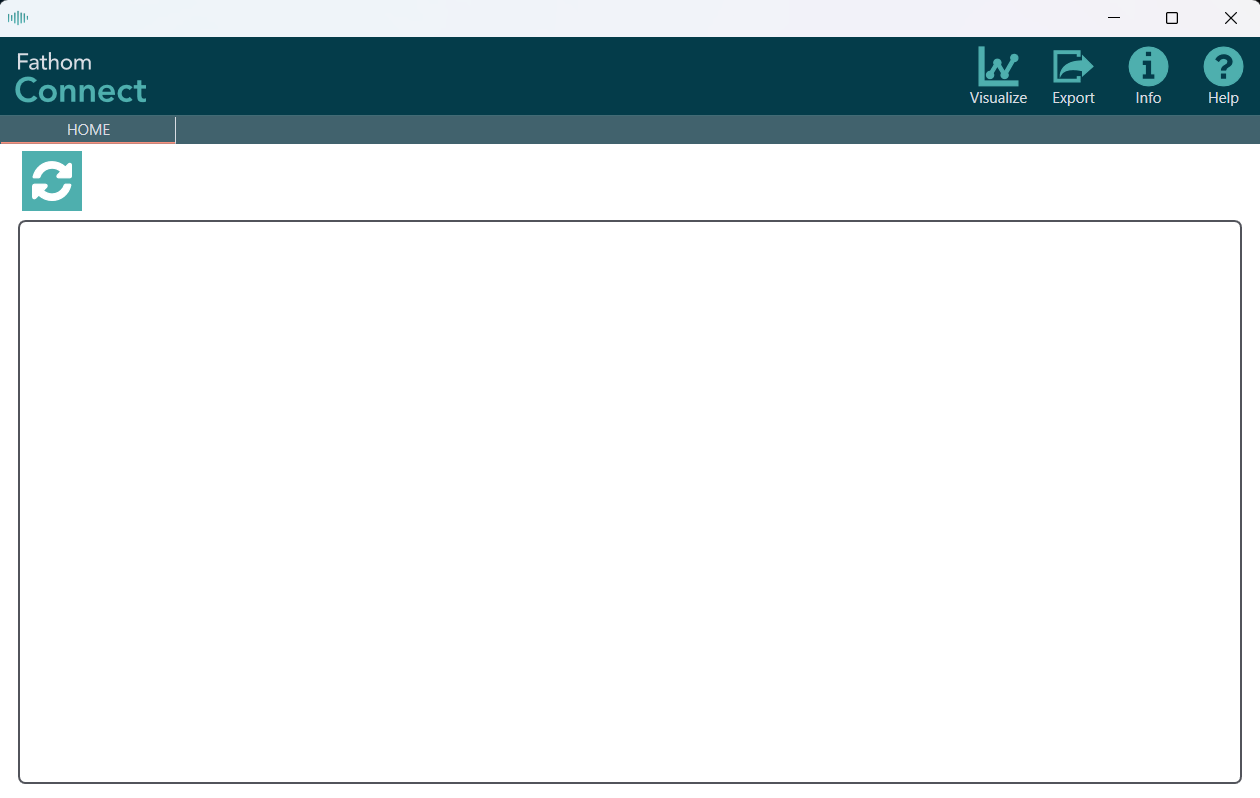
\includegraphics{images/fathom/home.png}

Click the ``refresh'' button in the top-left of the screen to scan for
receivers. It is likely that you will have to do this more than once to
pick up the receiver. A tile will appear when the receiver has been
identified:

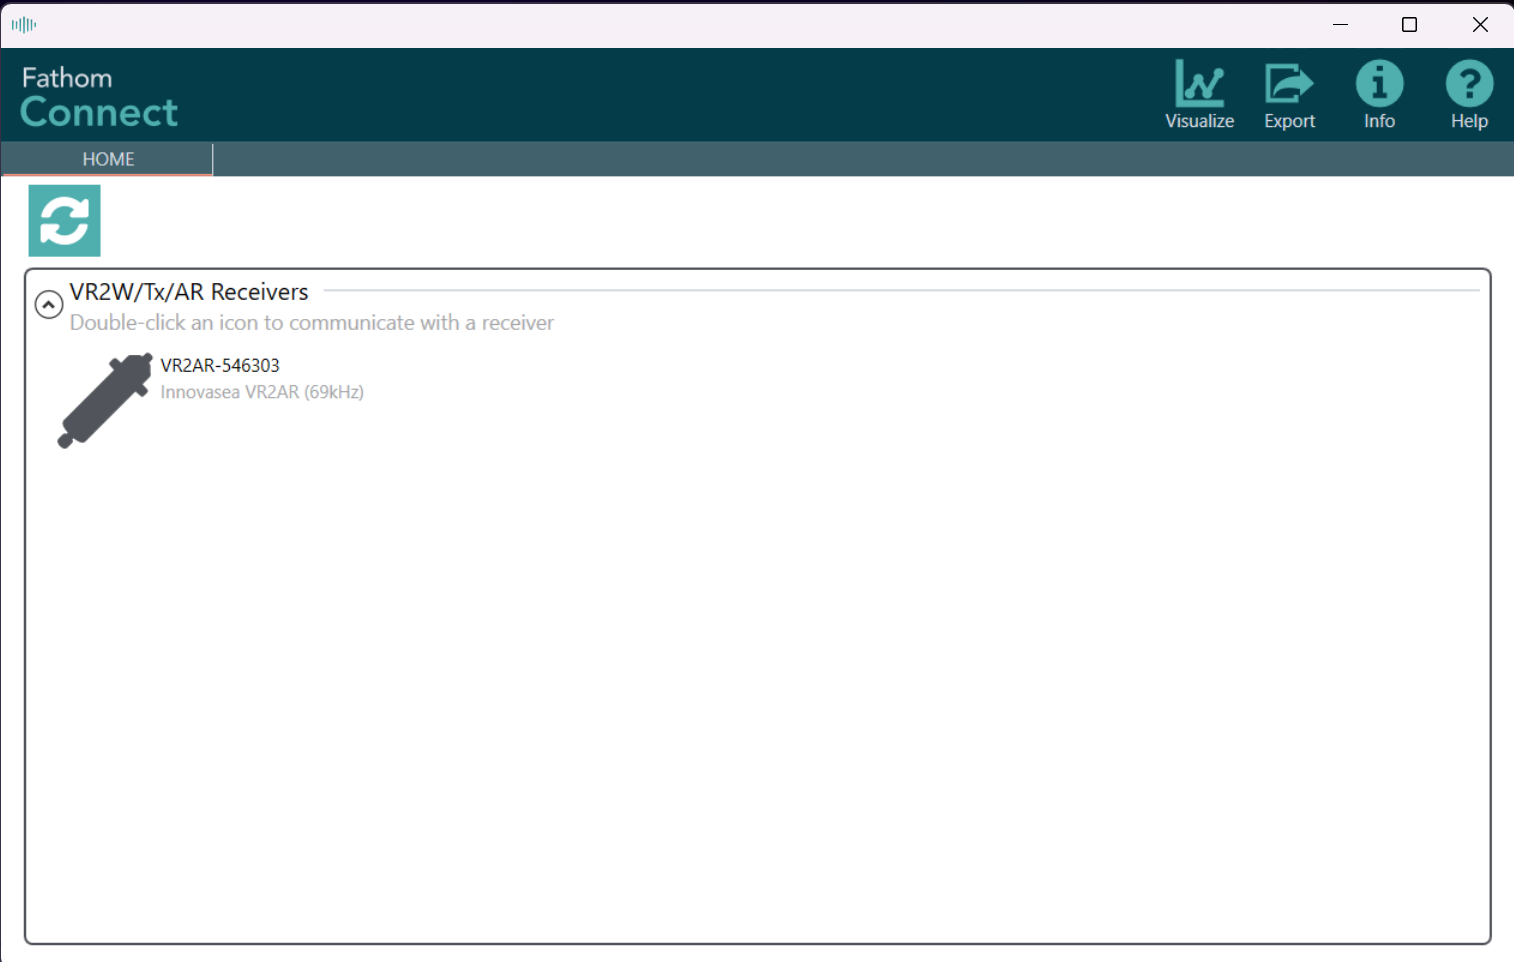
\includegraphics{images/fathom/home_with_rec.png}

Double click on the receiver.

\section{Firmware updates}\label{firmware-updates}

If you have updated Fathom Connect since the last time you connected to
your receiver, you will likely be greeted with a window warning you that
a new firmware version is available.

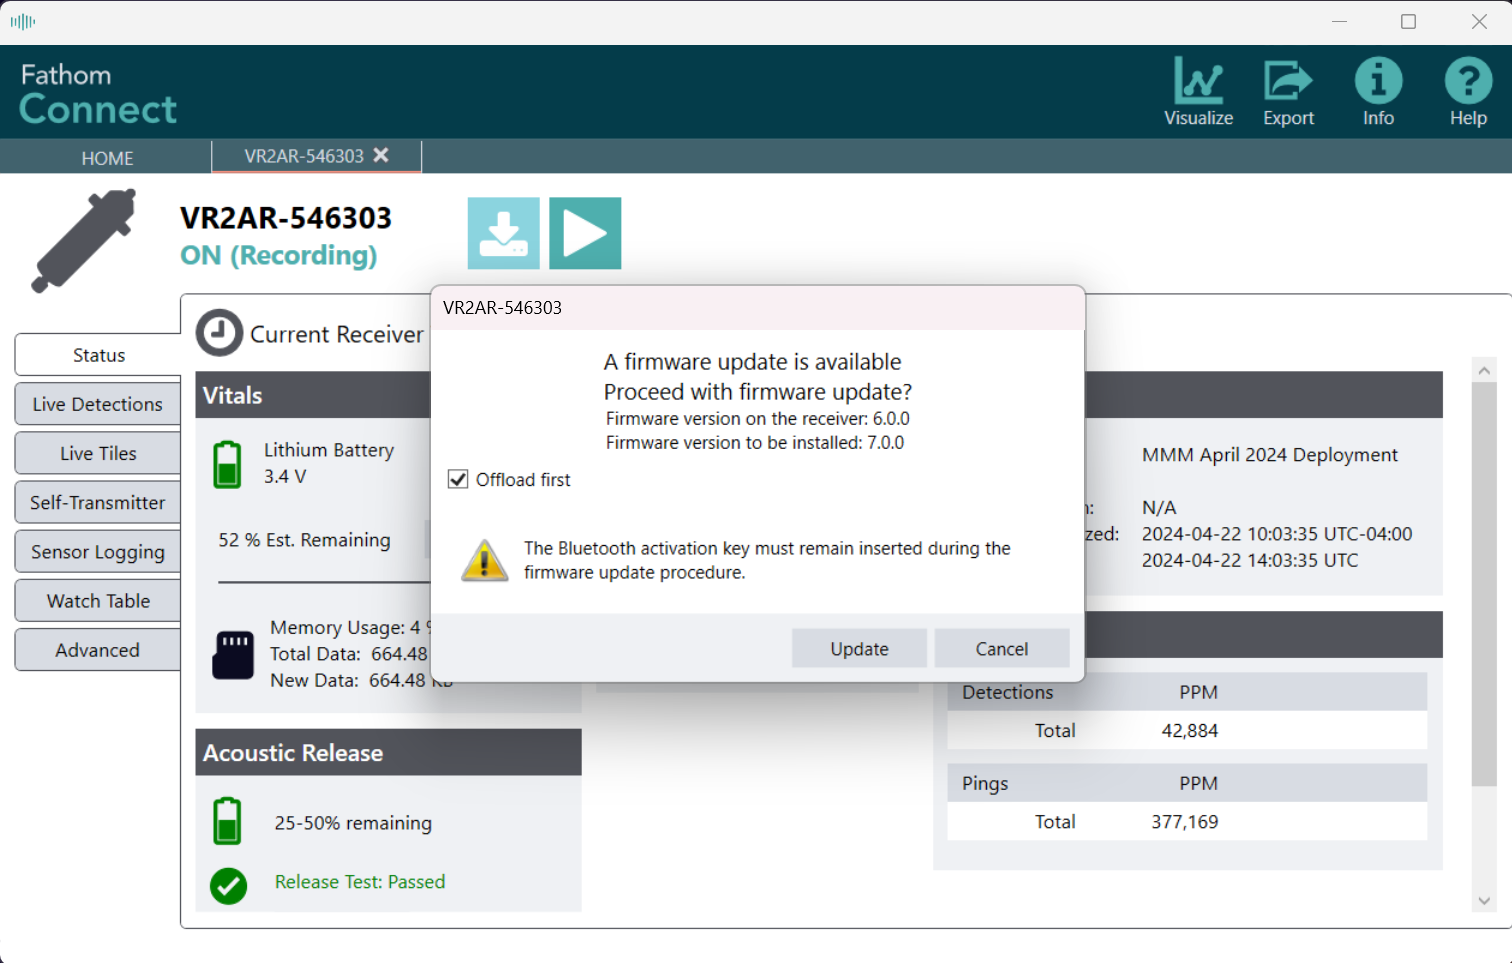
\includegraphics{images/fathom/firmware_notice.png}

\begin{tcolorbox}[enhanced jigsaw, title=\textcolor{quarto-callout-important-color}{\faExclamation}\hspace{0.5em}{Important}, leftrule=.75mm, colback=white, colframe=quarto-callout-important-color-frame, opacityback=0, toptitle=1mm, titlerule=0mm, colbacktitle=quarto-callout-important-color!10!white, toprule=.15mm, left=2mm, bottomtitle=1mm, arc=.35mm, breakable, coltitle=black, rightrule=.15mm, bottomrule=.15mm, opacitybacktitle=0.6]

Updating firmware will delete everything on your receiver!

Make sure the ``Offload first'' box is ticked to save data on the
receiver before updating the firmware.

\end{tcolorbox}

\section{Offloading data}\label{offloading-data}

If you were not prompted to update receiver firmware, you will land on
the receiver's \textbf{Status} page. This provides information on
battery usage (both CPU and release battery if connected to an
acoustic-release receiver), memory usage, connection type (Bluetooth or
cabled), internal transmitter status, study metadata, and logged
detections and pings.

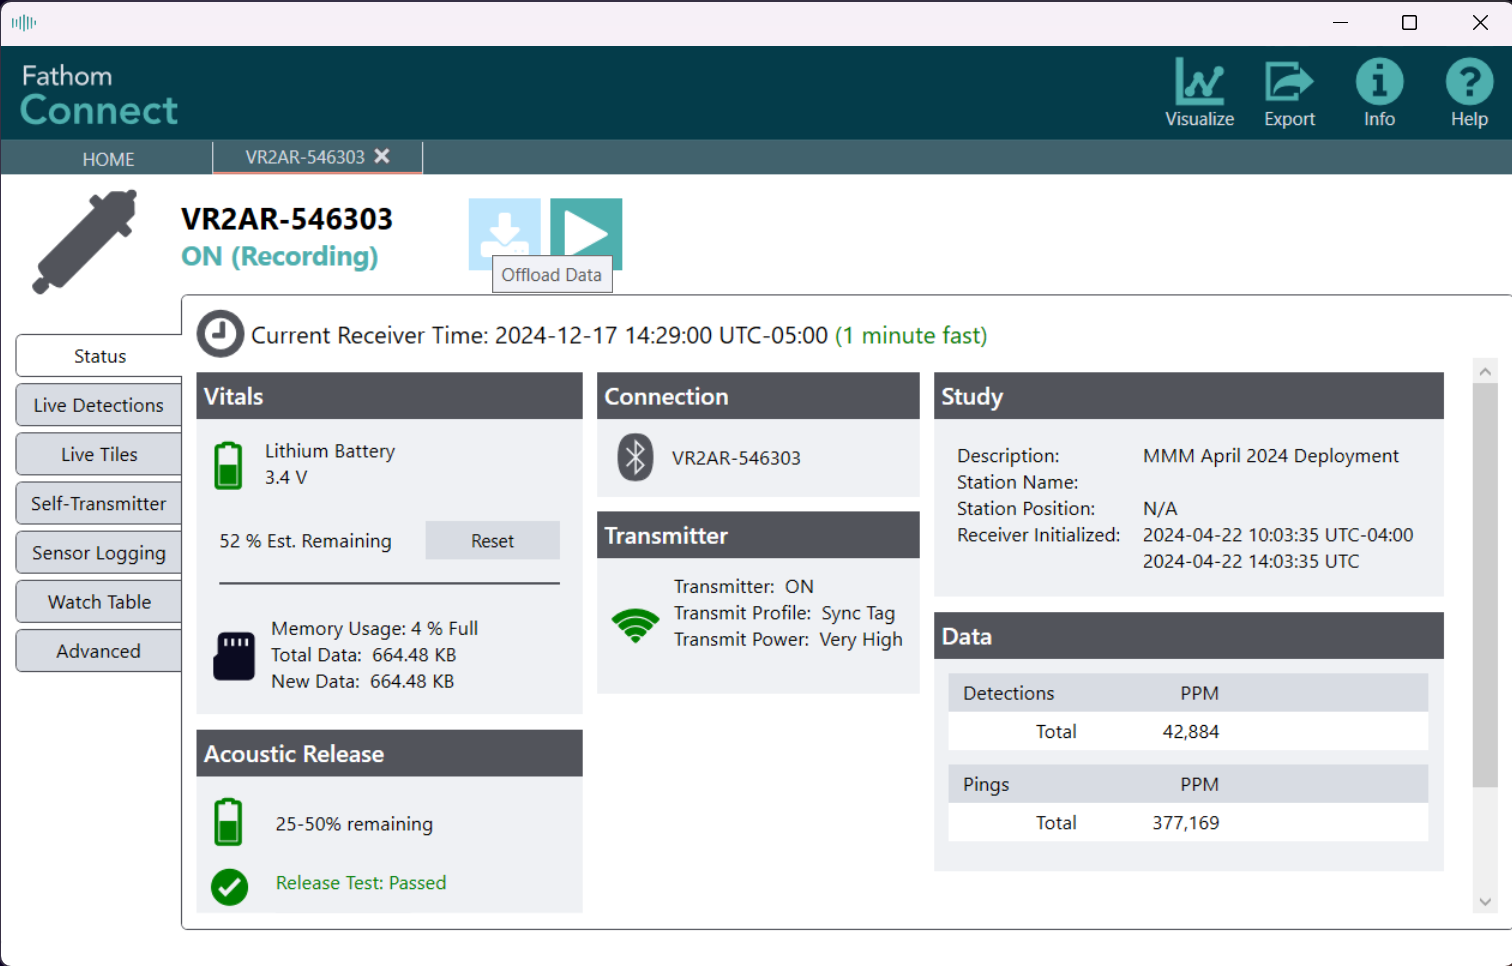
\includegraphics{images/fathom/status_page.png}

To offload data, click the ``download'' button near the top-left of the
screen.

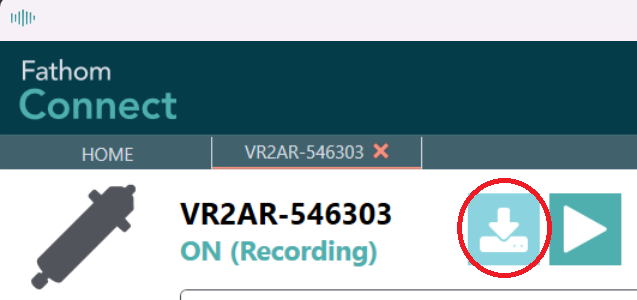
\includegraphics{images/fathom/buttons_download.png}

A pop-up will appear asking where you would like the file to be saved
and whether you want to offload all data or just new data. Adjust
settings and click ``Start''.

\begin{tcolorbox}[enhanced jigsaw, title=\textcolor{quarto-callout-tip-color}{\faLightbulb}\hspace{0.5em}{Tip}, leftrule=.75mm, colback=white, colframe=quarto-callout-tip-color-frame, opacityback=0, toptitle=1mm, titlerule=0mm, colbacktitle=quarto-callout-tip-color!10!white, toprule=.15mm, left=2mm, bottomtitle=1mm, arc=.35mm, breakable, coltitle=black, rightrule=.15mm, bottomrule=.15mm, opacitybacktitle=0.6]

I suggest always selecting ``Offload All Data'' to hedge against data
loss by having redundant records.

\end{tcolorbox}

\begin{tcolorbox}[enhanced jigsaw, title=\textcolor{quarto-callout-note-color}{\faInfo}\hspace{0.5em}{Note}, leftrule=.75mm, colback=white, colframe=quarto-callout-note-color-frame, opacityback=0, toptitle=1mm, titlerule=0mm, colbacktitle=quarto-callout-note-color!10!white, toprule=.15mm, left=2mm, bottomtitle=1mm, arc=.35mm, breakable, coltitle=black, rightrule=.15mm, bottomrule=.15mm, opacitybacktitle=0.6]

Files are saved to
\texttt{C:\textbackslash{}Users\textbackslash{}USERNAME\textbackslash{}Documents\textbackslash{}Innovasea\textbackslash{}Fathom\textbackslash{}YYYY-mm-DD},
where ``USERNAME'' is your computer's user name and ``YYYY-mm-DD'' is
today's date. The ``YYYY-MM-DD'' portion will be automatically created
in the listed directory.

\end{tcolorbox}

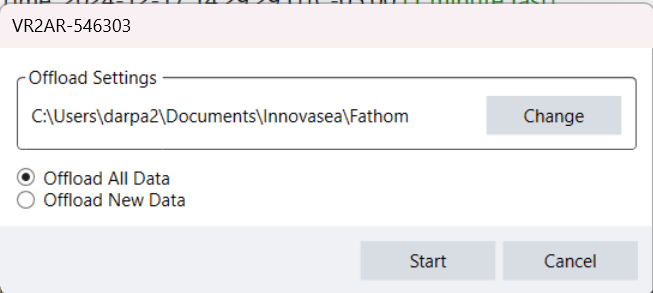
\includegraphics{images/fathom/offload_info.png}

Fathom Connect will ask you to confirm that your computer's time is
correct. If your computer has been connected to the internet for a few
minutes, click ``OK''.

\begin{tcolorbox}[enhanced jigsaw, title=\textcolor{quarto-callout-warning-color}{\faExclamationTriangle}\hspace{0.5em}{Warning}, leftrule=.75mm, colback=white, colframe=quarto-callout-warning-color-frame, opacityback=0, toptitle=1mm, titlerule=0mm, colbacktitle=quarto-callout-warning-color!10!white, toprule=.15mm, left=2mm, bottomtitle=1mm, arc=.35mm, breakable, coltitle=black, rightrule=.15mm, bottomrule=.15mm, opacitybacktitle=0.6]

If your computer has not been connected to the internet for some time,
it has likely experienced clock drift (yes, like a receiver!!). Before
proceeding, you should confirm your time with a clock that has been
connected to the internet (your phone, another computer, etc.).

\end{tcolorbox}

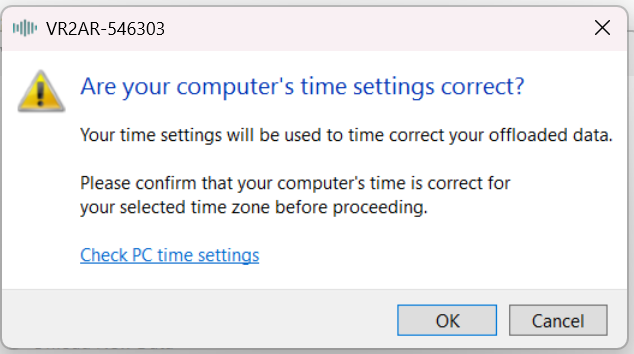
\includegraphics{images/fathom/time_warning.png}

You will be shown a progress window, culminating in (hopefully) a
notification of success!

Note that the file name is of the form
\texttt{MODEL-KHZ\ SERIAL\ YYYY-mm-DD\ HHMMSS.vdat}, spaces included.

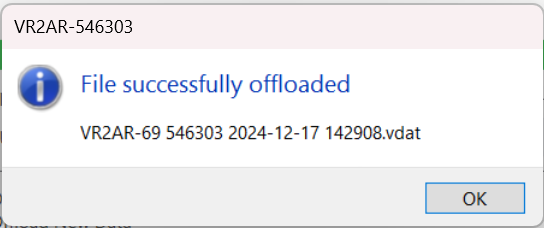
\includegraphics{images/fathom/offload_success.png}

Navigate to the file location to confirm that the file has been
downloaded and is where you think it is. By default, the file downloaded
above went to
\texttt{C:\textbackslash{}Users\textbackslash{}MYUSERNAME\textbackslash{}Documents\textbackslash{}Innovasea\textbackslash{}Fathom\textbackslash{}2024-12-17}
as it was created on December 17, 2024.

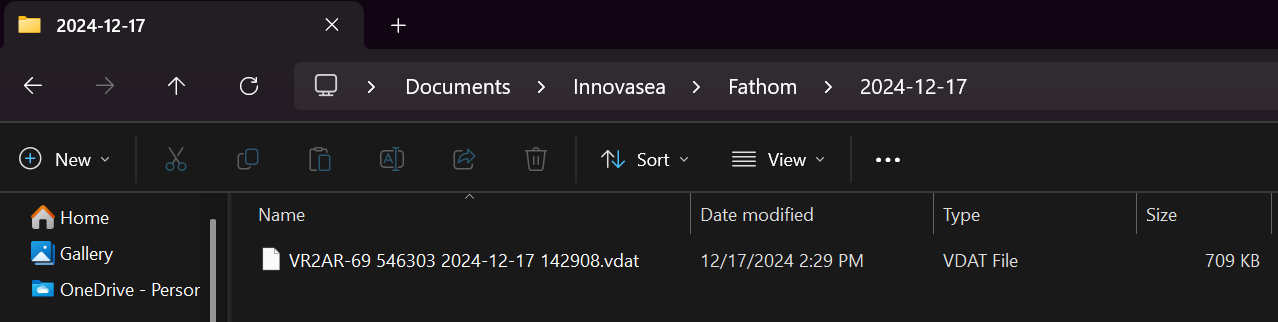
\includegraphics{images/fathom/file_location.png}

\section{Internal transmitter}\label{internal-transmitter}

\subsection{Long-term detection range}\label{long-term-detection-range}

If multiple receivers are planned to be deployed within ``earshot'' of
each other (generally within 200-800 meters, environment-dependent) and
your receiver has the capability (anything that isn't a VR2W), it is
worthwhile to activate the internal transmitter in order to characterize
detection range during the receiver's future deployment.

Select the \textbf{Sync Tag} option. This will emit the receiver's
programmed transmitter ID every ten minutes, on average.

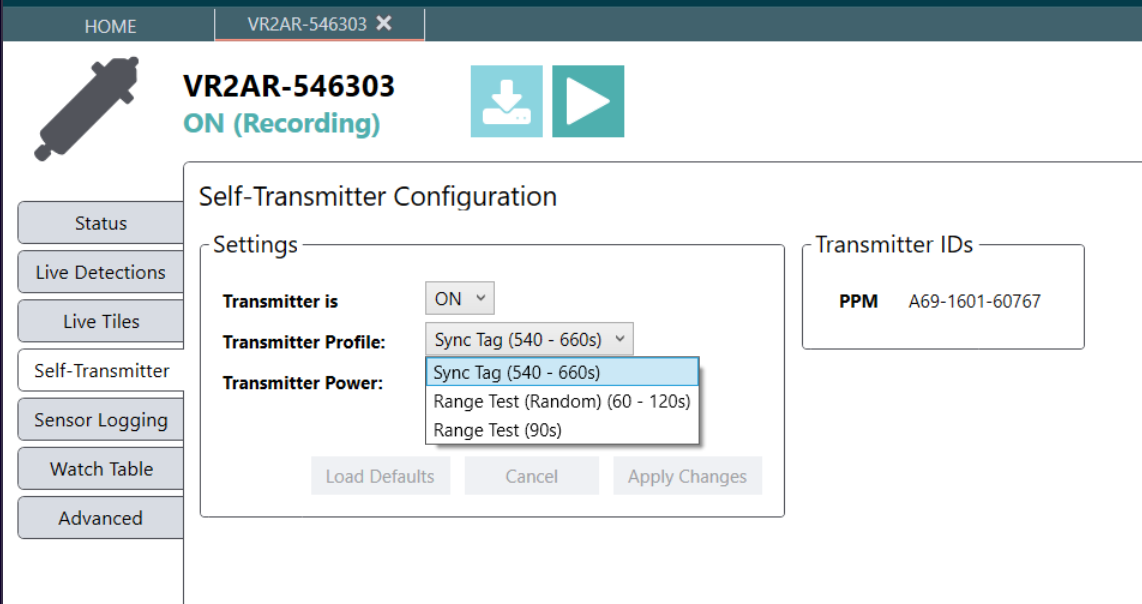
\includegraphics{images/fathom/self_transmitter_profile.png}

Select a power level that is comparable to the targeted transmitters,
listed below.

\begin{tcolorbox}[enhanced jigsaw, title=\textcolor{quarto-callout-note-color}{\faInfo}\hspace{0.5em}{Note}, leftrule=.75mm, colback=white, colframe=quarto-callout-note-color-frame, opacityback=0, toptitle=1mm, titlerule=0mm, colbacktitle=quarto-callout-note-color!10!white, toprule=.15mm, left=2mm, bottomtitle=1mm, arc=.35mm, breakable, coltitle=black, rightrule=.15mm, bottomrule=.15mm, opacitybacktitle=0.6]

At the time of this writing, the most commonly-deployed transmitters are
V16s; the power level should be set to ``High'' or ``Very High'', with a
preference to ``Very High'' as most studies utilize high power to
increase detectability.

\end{tcolorbox}

\begin{itemize}
\tightlist
\item
  Very High = 160 dB
\item
  High = 154 dB
\item
  Medium = 148 dB
\item
  Low = 142 dB
\end{itemize}

Transmitter power:

\begin{itemize}
\tightlist
\item
  V16 = 152-162 dB re 1 \(\mu\)Pa @ 1m
\item
  V13 = 147-152 dB re 1 \(\mu\)Pa @ 1m
\item
  V9 = 146-151 dB re 1 \(\mu\)Pa @ 1m
\item
  V8 = 144-147 dB re 1 \(\mu\)Pa @ 1m
\item
  V7 and V6 = 137-141 dB re 1 \(\mu\)Pa @ 1m
\end{itemize}

\begin{tcolorbox}[enhanced jigsaw, title=\textcolor{quarto-callout-note-color}{\faInfo}\hspace{0.5em}{Note}, leftrule=.75mm, colback=white, colframe=quarto-callout-note-color-frame, opacityback=0, toptitle=1mm, titlerule=0mm, colbacktitle=quarto-callout-note-color!10!white, toprule=.15mm, left=2mm, bottomtitle=1mm, arc=.35mm, breakable, coltitle=black, rightrule=.15mm, bottomrule=.15mm, opacitybacktitle=0.6]

Internal transmitter power is not provided at a reference distance and
pressure -- this is purposeful, as these are not calibrated values and
could be off depending on anything from manufacturing variation to the
deployed environment. Because of this, we're just trying to get in the
correct range rather than trying to exactly match any values.

\end{tcolorbox}

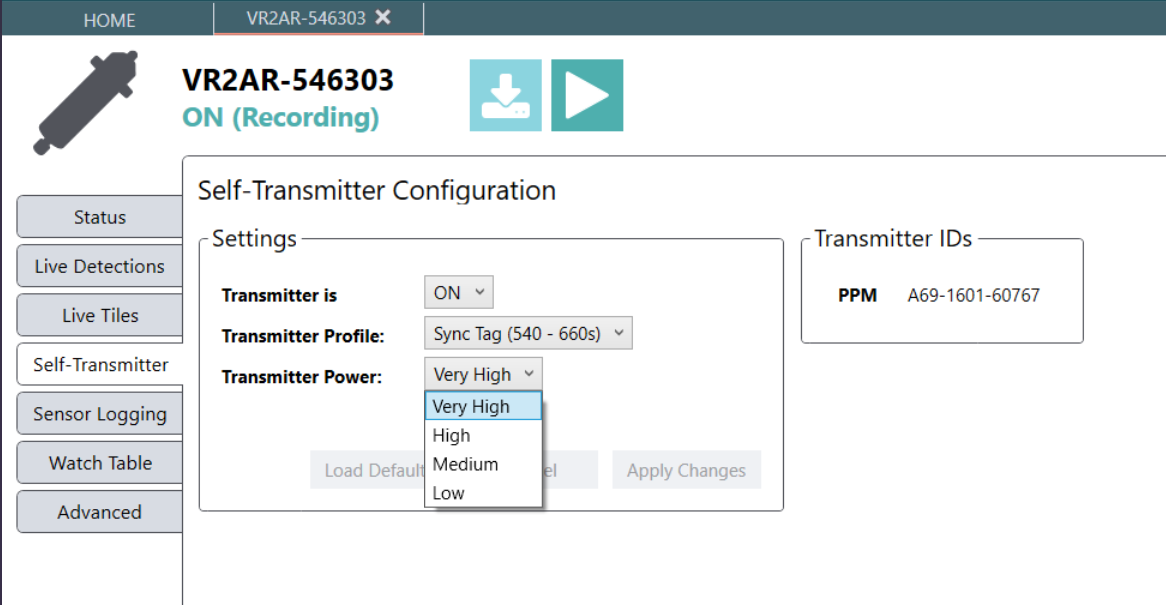
\includegraphics{images/fathom/self_transmitter_power.png}

\section{Study configuration}\label{study-configuration}

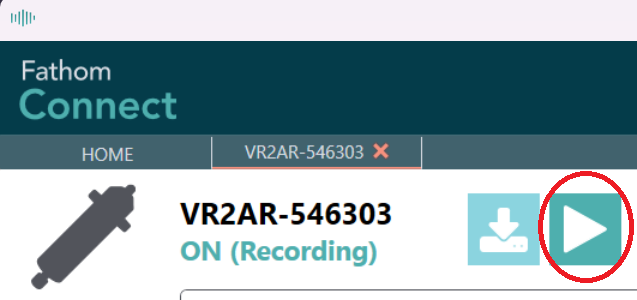
\includegraphics{images/fathom/buttons_config.png}

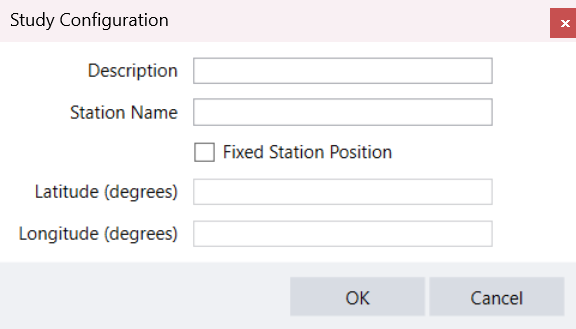
\includegraphics{images/fathom/study_config.png}

\section{Closing a session}\label{closing-a-session}

When everything is finished and you're ready to deploy the receiver (or
put it on the shelf), click the red X.

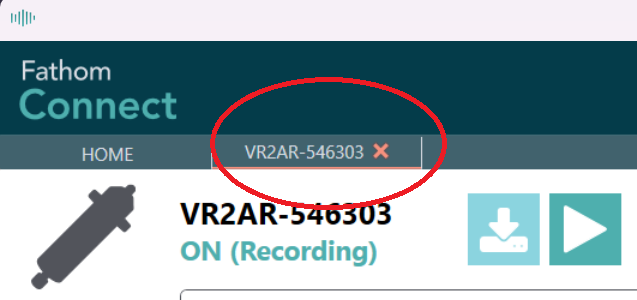
\includegraphics{images/fathom/buttons_exit.png}

\bookmarksetup{startatroot}

\chapter{Acoustic Release Deployment and
Recovery}\label{acoustic-release-deployment-and-recovery}

\bookmarksetup{startatroot}

\chapter{Receiver Transport and
Storage}\label{receiver-transport-and-storage}

\bookmarksetup{startatroot}

\chapter*{References}\label{references}
\addcontentsline{toc}{chapter}{References}

\markboth{References}{References}

\phantomsection\label{refs}
\begin{CSLReferences}{0}{1}
\end{CSLReferences}




\end{document}
